\chapter{Waypoint-sampling based motion planning}\label{cha:motion_planning_fw}
\section{Waypoint sampling}
The desired output of the motion planner in this thesis is a waypoint sequence $\mathcal{M}$, as defined in section \ref{sec:mission},
which takes the \ac{uav} from a desired initial position and heading $(\vec{p}_0,\psi_0)$ to a goal position and heading $(\vec{p}_g,\psi_u)$. Moreover, physical constraints of the \ac{uav} and wind should be taken into account. This formulation is well aligned with \textit{input sampling} methods such as Hybrid $A^*$ \cite{hybrid_astar}. 
In such methods, the reachability graph is created by forward simulation of the transition function $f(x, u)$ using input values $u$ sampled from a 
set $\inputs$. 

\subsection{State and input set definition}
Based on the kinematic model in Equation \eqref{eq:traj_model} the state vector is defined as
\begin{equation}
    x=(x_N, y_E, \psi)
\end{equation}
The input is defined as 
\begin{equation}
    u=\vec{p}_{i+1}-\vec{p}_i\equiv(\Delta x_N, \Delta y_E)
\end{equation}
\ie\ the coordinates of the next waypoint relative to the current, specified in the inertial frame.
\subsection{State transition function}
The definition of $u$ combined with the trajectory following controller derived in Section \ref{sec:traj_controller} 
leads to a model of the closed-loop system. Using such a model during forward simulation, 
guarantees in theory that the controller will be able to track the resulting reference trajectory. 

The desired \ac{cog} for the current line-segment is
\begin{equation}
    \psi_u=\atan2(\Delta y_E,\Delta x_N)
\end{equation}
If roll dynamics are neglected, the commanded rate of turn is obtained by inserting the roll command from Equation \eqref{eq:roll_cmd} into Equation \eqref{eq:traj_model}, which gives 
\begin{equation}
    \dot{\psi}_{\text{cmd}}=\frac{a_{\text{cmd}}}{\airspd}
\end{equation}
where $a_{\text{cmd}}$ is given by Equation \eqref{eq:lat_acc} with $\eta$ as defined in \eqref{eq:eta_first}--\eqref{eq:eta_last}.
However, for a real \ac{uav} the magnitude of the rate of turn is limited by some $\dot{\psi}_{\text{max}}$. The actual value of $\dot{\psi}$ is thus
\begin{equation}\label{eq:saturation}
    \dot{\psi}=\begin{cases}
        \dot{\psi}_{\text{cmd}} & |\dot{\psi}_{\text{cmd}}| \leq \dot{\psi}_{\text{max}} \\
        \text{sgn}(\dot{\psi}_{\text{cmd}})\dot{\psi}_{\text{max}} & \text{otherwise}
    \end{cases}
\end{equation}
Finally, the kinematic model of the closed-loop system becomes
\begin{equation}\label{eq:closed_loop}
    \dot{x}=f(x,u)=
    \begin{bmatrix}
        V_E\\
        V_N\\
        \dot{\psi}
    \end{bmatrix}
\end{equation}

\section{Input set generation}\label{sec:motion_prims_wind}
An input set $\inputs$ is a subset of a motion primitive set $\mathcal{P}$ introduced in Section \ref{sec:motion_prim}. Therefore, 
the heading-change method introduced in \cite{Bergman_lic} to generate $\mathcal{P}$ can also be applied for generating $\inputs$. The resulting inputs will consist
of waypoints that result in a desired change of heading while taking \ac{uav} kinematics, wind and tracking performance of the controller into account.

\subsection{Optimal control formulation}
The input set is generated by solving the optimal control problem
\begin{subequations}
    \label{eq:opt_problem_mp_uav}
    \begin{alignat}{3}
    &\min_{x(t),u,T}        &\qquad& J=\Phi(x(T),u) + \int_{0}^{T}\airspd dt & \\
    &\text{subject to} & & \psi(0)=\wca &\\
    & & & |\cog(x(T))-\Delta\cog| \leq \Delta\psi_{\text{min}} &\\
    & & & \dot{x}=f(x(t), u) &\\
    & & & x(t)\in\states& \\
    & & & u\in\actions &
    \end{alignat}
\end{subequations}
for different values of $\windvec$ and course change $\Delta\cog$. To increase the feasible region, the constraint on $\cog(x(T))$ is relaxed to allow values in a region around the desired $\Delta\cog$ 
instead of a strict equality constraint. The closed-loop kinematic model \eqref{eq:closed_loop} depends on wind, which has to be taken into account when generating $\inputs$. This dependency as well as other relevant properties of \eqref{eq:opt_problem_mp_uav} are discussed in the sections below.

\subsubsection{Discretization of the wind direction}
During motion planning in wind, the heading relative to the wind $\psi_r=\psi-\winddir$ might take on any value.
In practice, this implies that inputs must be generated for a set of discrete wind directions $\{\psi_{r,0},\hdots,\psi_{r,n}\}$ which have to cover 360 degrees. 
Given a relative heading
\begin{equation}
    \psi_r: \psi_{r,i}<\psi_r<\psi_{r,i+1}
\end{equation}
the input $u\in\inputs$ selected by the planning algorithm was generated for $\psi_{r,i}$ or $\psi_{r,i+1}$. The discretization interval $|\psi_{w,i+1}-\psi_{w,i}|$ has to be sufficiently small
in order to secure good tracking performance of the closed-loop system.

\subsubsection{Planning with \ac{cog} instead of heading}
As shown in Section \ref{sec:straight_path_wind}, the heading required to follow a line-segment is dependent on the current wind $\windvec$. 
Therefore constraints related to direction change in Equation~\eqref{eq:opt_problem_mp_uav} are formulated in terms of $\cog$ as defined in Equation~\eqref{eq:cog}.
A direct consequence is that the initial value of $\psi$ when generating inputs should be 
set to $\wca$ defined in Equation \eqref{eq:wca}, as this corresponds to an initial $\cog$ of $0\degree$.

\subsubsection{Cross-track error penalty}
The cross-track error at the end of a line-segment can be calculated as 
\begin{equation}
    d(x(T), u) = x_{N}(T)\sin\psi_u-y_{E}(T)\cos\psi_u
\end{equation}
If $d(x(T), u)\neq0$ the initial cross-track error for the next line-segment will be non-zero. 
Since the closed-loop system is used when expanding the graph, a small initial error can be mitigated.
The cross-track error penalty is defined as
\begin{equation}\label{eq:phi_d}
    \Phi(x(T), u)=\lambda_d\max(|d(x(T), u)|-d_{\text{min}},0)
\end{equation}
and is included in the optimization objective \eqref{eq:opt_problem_mp_uav}. 
This term is, by construction, zero when the final cross-track error is below some acceptable threshold $d_{\text{min}}$. In this case, only the trajectory length is penalized. 
The penalty for larger cross-track errors is tuned by the scaling factor $\lambda_d>0$.

\subsection{Solving the optimal control problem}
Methods commonly used to solve optimal control problems include \textit{multiple shooting} 
and \textit{direct collocation} \cite{multiple_shooting}. 
However, the following properties of \eqref{eq:opt_problem_mp_uav} makes it hard to solve with such methods:
\begin{enumerate}
    \item The closed-loop system is highly non-linear, especially when including the saturation from Equation \eqref{eq:saturation}.
    \item In optimal control problems the input $u(t)$ can normally be chosen freely from $\actions$ for each time-step, while 
    in this formulation the input is forced to be a constant $u(t)=u$, $0<t<T$.
\end{enumerate}
The second property implies that when transformed to a Nonlinear Program using \eg\ multiple shooting,
the optimization variables corresponding to $x(t)$ in each time-step all depend on the same constant $u$. In this sense the resulting formulation is 
more closely related to a \textit{direct shooting} problem, which are known to be less linear and thus harder to solve \cite{multiple_shooting}.

\subsubsection{Derivative-free Optimization}
Since all properties of the solution of Equation \eqref{eq:opt_problem_mp_uav} are dependent on the choice of $u$, different solutions can be studied by simulating
the closed-loop system for different choices of $u$. Choices of $u$ which lead to solutions that violate the constraints 
can easily be pruned. A number of solutions with different characteristics for a desired course change $\Delta\cog=90\degree$ are illustrated in Figure~\ref{fig:opt_contour}. 

\begin{figure}
    \subfloat[$u=(90,140)$: Infeasible solution due to incorrect final $\cog$.]{
        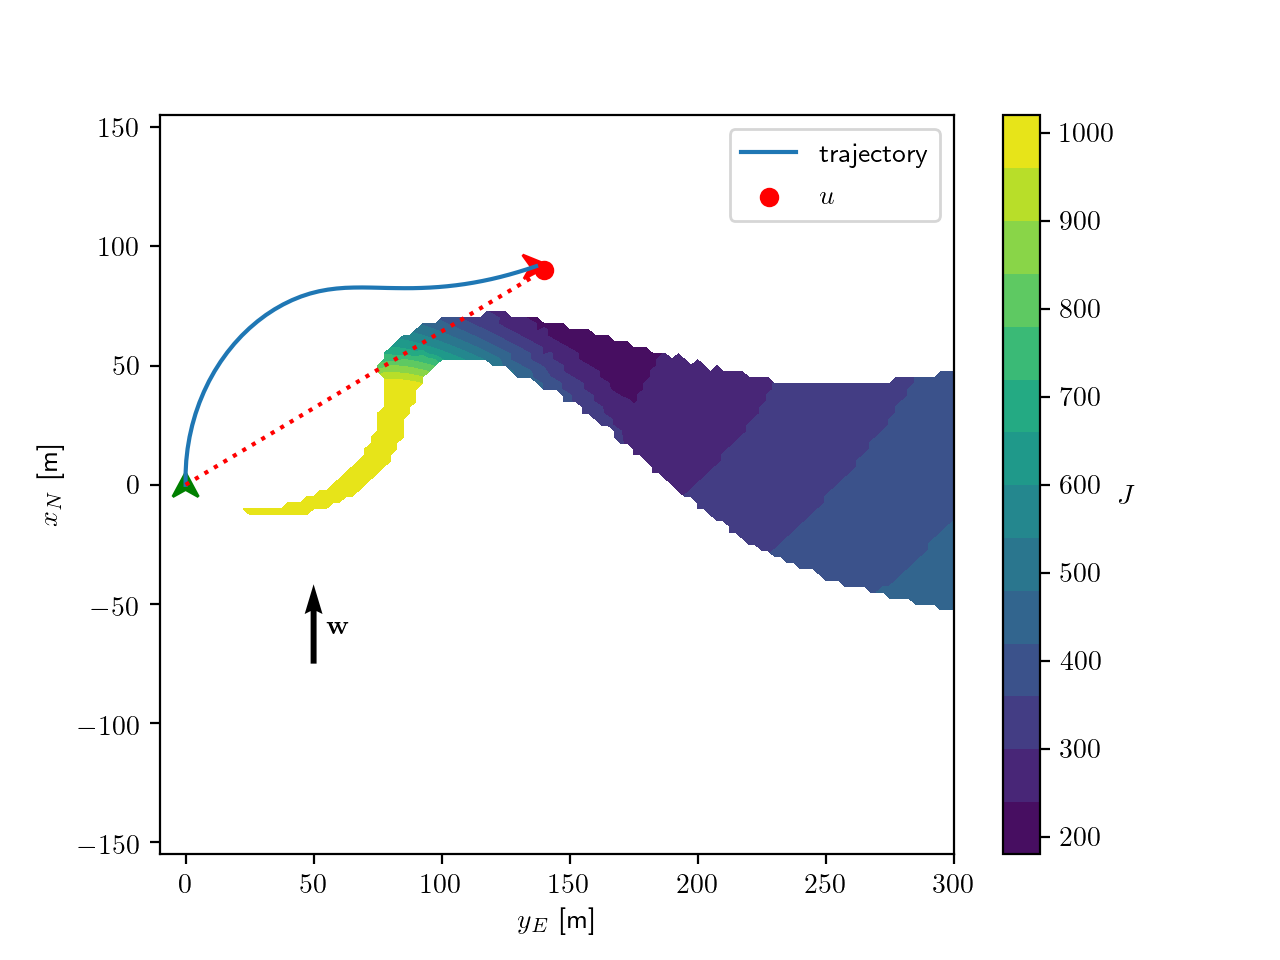
\includegraphics[width=.48\linewidth]{J_sim_90_140}
    }
    \subfloat[$u=(50,90)$: Sub-optimal solution due to large final cross-track error, $J=891$.]{
        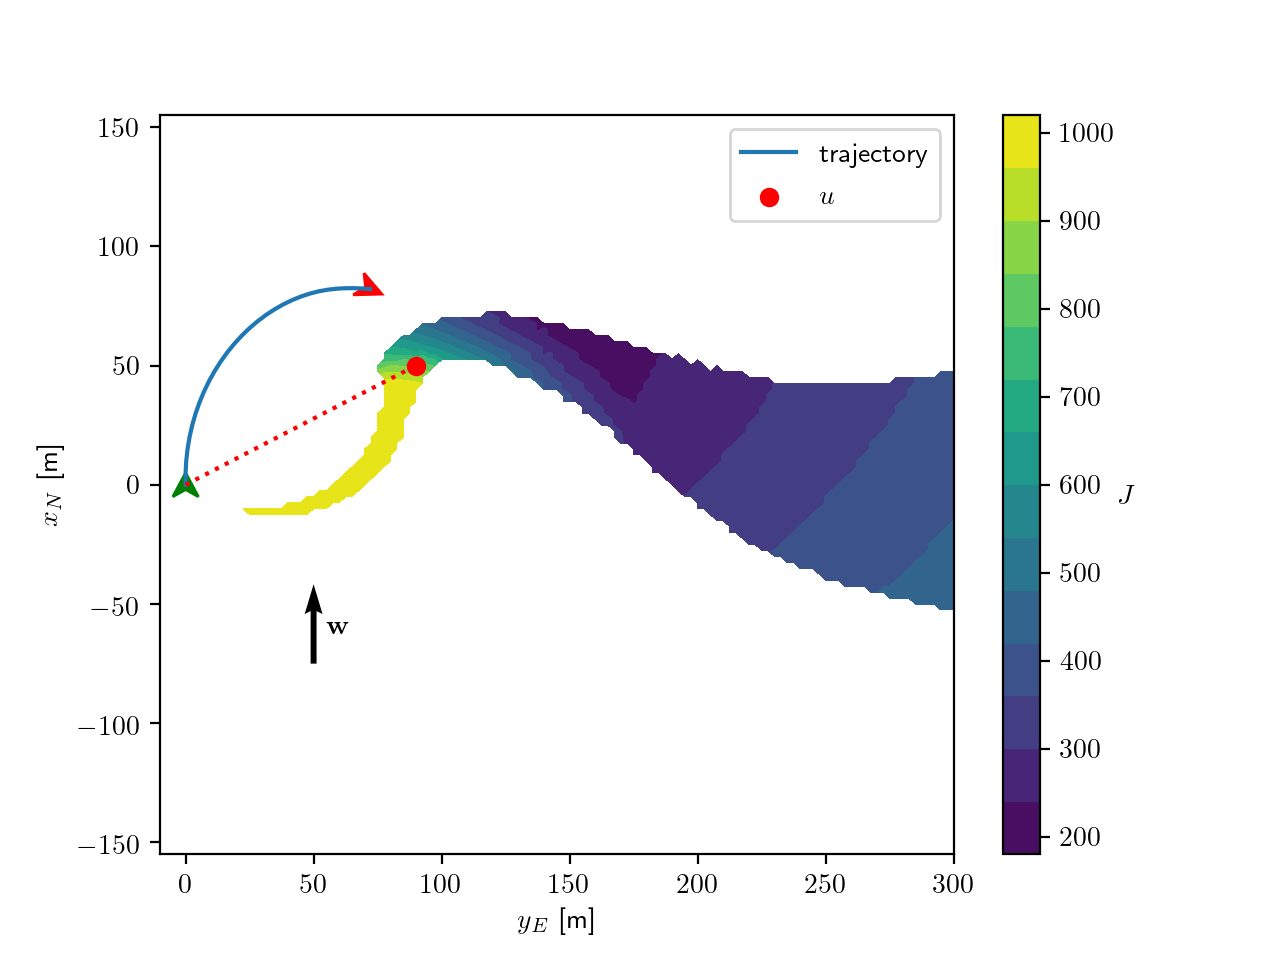
\includegraphics[width=.48\linewidth]{J_sim_50_90}
    }\\
    \subfloat[$u=(-10,280)$: Sub-optimal solution due to unnecessarily long trajectory, $J=378$.]{
        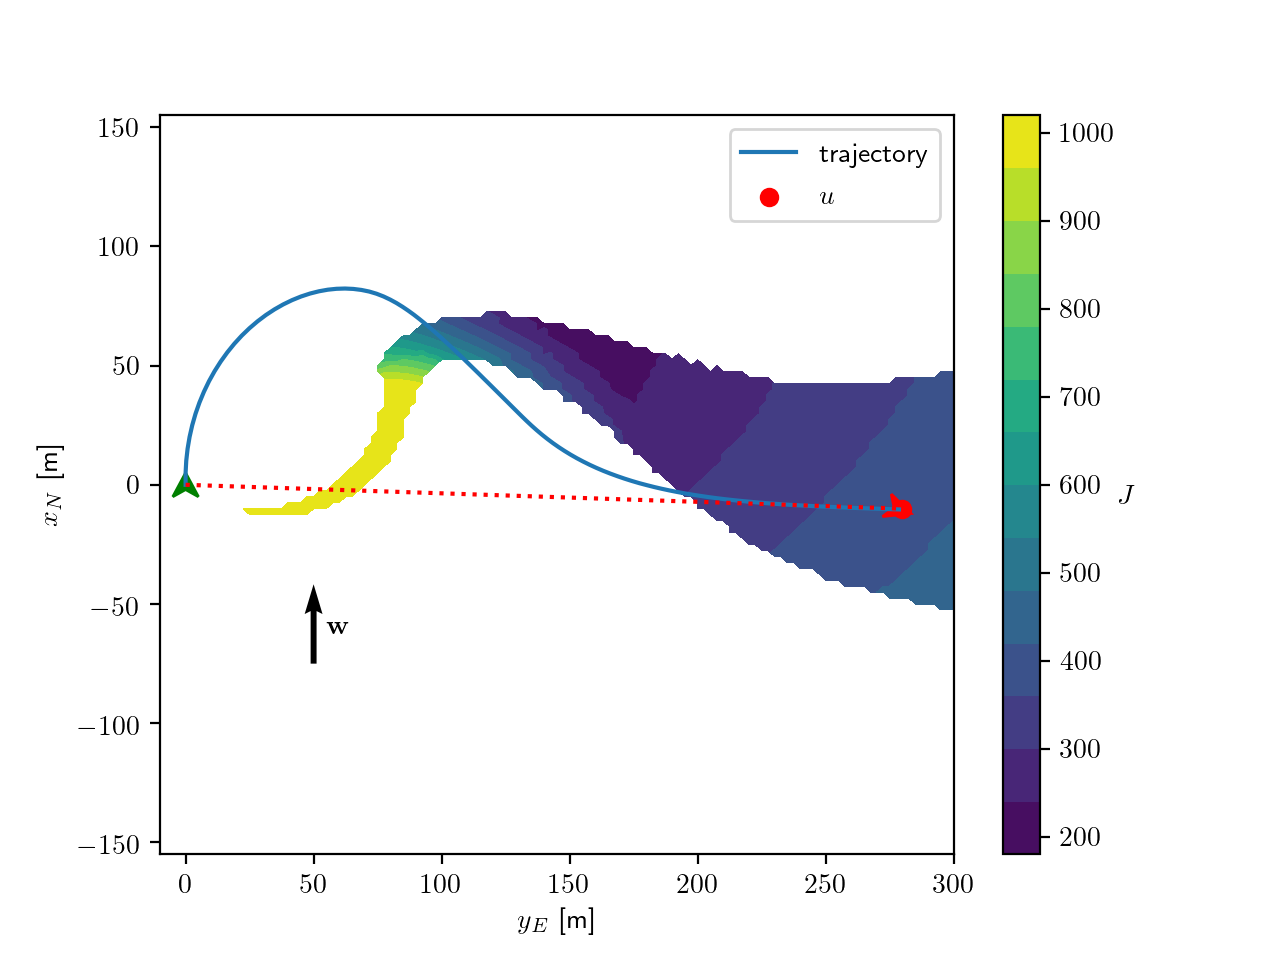
\includegraphics[width=.48\linewidth]{J_sim_10_280}
    }
    \subfloat[$u=(67,147)$: Optimal solution, $J=186$.]{
        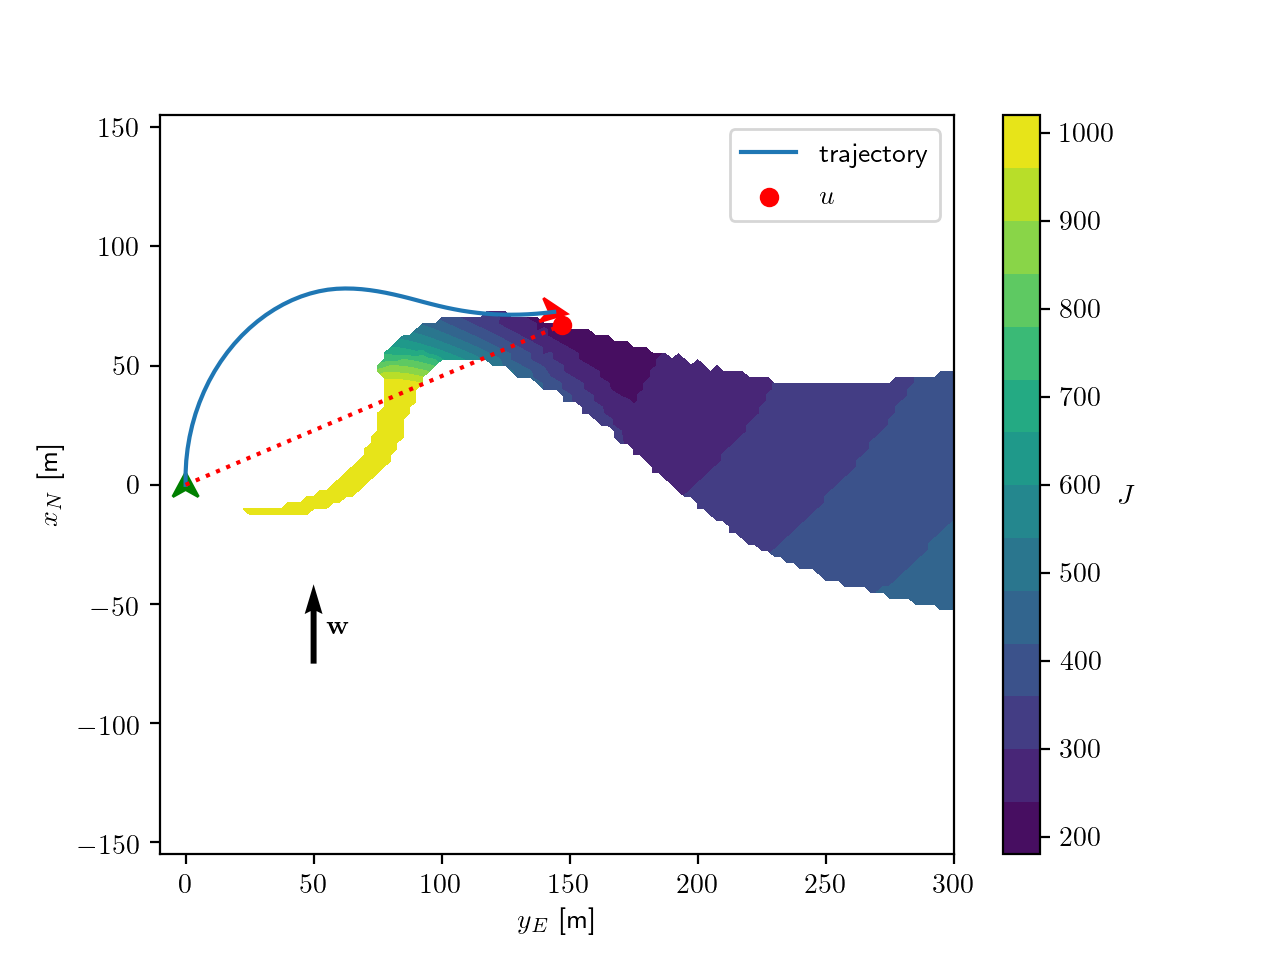
\includegraphics[width=.48\linewidth]{J_sim_67_147}
    }
    \caption{Solutions of \eqref{eq:opt_problem_mp_uav} for different values of $u$, for desired course change $\Delta\cog=90\degree$, $\Delta \psi_{\text{max}}=10\degree$ and $\lambda_d=25$. The colored area represents values of $u$ which 
    lead to feasible solutions. Brighter colors represent higher values of the objective function $J$. The green and red arrows represent initial and final states of the \ac{uav}. The wind was defined as $\windspd=5$ m/s and $\winddir=0\degree$.}
    \label{fig:opt_contour}
\end{figure}

As can be seen the feasible region is non-convex but there is a clear global optimum. Since there are only two free parameters, the north and east coordinates of $u$, 
an approximate optimum could be found by performing a grid search over different values of these parameters. However, this solution would depend on the discretization interval of the grid 
and searching over a grid with sufficiently fine resolution is computationally expensive.
A more efficient method is to use \textit{derivative-free} optimization methods, as presented in \cite{derivative_free_opt}. 
In those methods the optimization problem is formulated as 
\begin{subequations}
    \label{eq:derivative_free_opt}
    \begin{alignat}{3}
    &\min_{\xi\in\reals^n}        &\qquad& F: \xi \rightarrow \reals & \\
    &\text{subject to} & & \xi\in\Omega\subseteq \reals^n&\\
    \end{alignat}
\end{subequations}
where no other information, such as the derivatives of $F$, is available.
One class of derivative-free methods called \ac{mads} was introduced in \cite{mads}. This method is based on creating an increasingly fine grid around the currently optimal 
solution on which the objective function is evaluated. In \cite{mads} this method is shown to successfully converge to the global optimum of various non-convex optimization problems using the derivative-free optimization formulation.

\subsection{Robustness during wind variations}
The requirement to generate a set of inputs for each possible wind speed limits 
the practical applicability of the method.
A more useful approach is to generate input sets which handle wind speeds 
$\windspd\in[W_{\text{min}},W_{\text{max}}]$. This problem can be formulated as finding an input $u$ which is feasible for both 
$W_{\text{min}}=(1-\delta_W)\Tilde{\windspd}$ and $W_{\text{max}}=(1+\delta_W)\Tilde{\windspd}$ for some $\delta_W<1$ and $\Tilde{\windspd}=(W_{\text{max}}-W_{\text{min}})/2$. 
Therefore, the derivative-free optimization problem was formulated as
\begin{subequations}
    \label{eq:max_opt}
    \begin{alignat}{3}
    &\min_{x, u}        &\qquad& F(x, u)=\max(J_{\text{low}}(x, u),J_{\text{high}}(x, u)) & \\
    &\text{subject to} & & (x, u)\in\Omega &\\
    \end{alignat}
\end{subequations}
where $J_{\text{low}}$ is the objective value of \eqref{eq:opt_problem_mp_uav} for $\windspd=W_{\text{min}}$ and $J_{\text{high}}$ is the objective value for $\windspd=W_{\text{max}}$. 
The feasible set $\Omega$ is defined as the values of $x$ and $u$ where the constraints in \eqref{eq:opt_problem_mp_uav} hold for all $\windspd\in[W_{\text{min}},W_{\text{max}}]$.

\section{Improvement step}
As mentioned in Section \ref{sec:hybrid-a-star} the initial solution from Hybrid $A^*$ is often improved using numerical optimization. 
However, due to the limitations presented above such methods are not available. Therefore, a simpler and practically motivated approach was used.

The initial solution computed by the Hybrid $A^*$ search is henceforth denoted
\begin{equation}
    \mathcal{M}_{\text{init}}=\{\vec{p}_0,\hdots,\vec{p}_n\}    
\end{equation}
which is an ordered sequence of $n$ waypoints $\vec{p}_i$. A sub-sequence of a mission is denoted
\begin{equation}
    \mathcal{M}_{k:l}=\{\vec{p}_k,\hdots,\vec{p}_l\}, \quad 0\leq k<l\leq n
\end{equation}
A \textit{reduced set} of waypoints is defined as 
\begin{equation}
    \mathcal{M}_{k,l}=\{\vec{p}_k,\vec{p}_l\}
\end{equation}
\ie\ the first and last waypoint of a sub-sequence $\mathcal{M}_{k:l}$. By simulating the closed-loop system using $\mathcal{M}_{\text{init}}$ the inital \ac{cog} and cross-track error $(\cog,d)_i$ at each waypoint can be recorded. 
Since \eqref{eq:closed_loop} minimizes the cross-track error in each timestep, the following relation always holds:
\begin{equation}
    L(\mathcal{M}_{l:k})\geq L(\mathcal{M}_{l,k})
\end{equation}
where $L(\cdot)$ denotes the length of the trajectory produced by simulating \eqref{eq:closed_loop} with a given waypoint sequence. If the same \ac{cog} and cross-track error 
is achieved and no obstacles are collided with while using $\mathcal{M}_{k,l}$ the intermediate waypoints of $\mathcal{M}_{k:l}$ can be eliminated. This method is outlined in Algorithm \eqref{alg:imp} where 
the function $\text{SIMULATE}(\mathcal{M},\xobst)$ returns the \ac{cog} and cross-track error achieved by simulating $\mathcal{M}$ and if there were any 
collissions with $\xobst$. The result of applying the improvement step to a Hybrid $A^*$ solution is illustrated in Figure~\ref{fig:imp}.

\begin{algorithm}
    \begin{algorithmic}
        \Require Initial mission $\mathcal{M}_{\text{init}}$ and corresponding \ac{cog} and cross-track errors $\{(\cog,d)_i\}$
        \State $\mathcal{M}_{\text{imp}}\gets \{\vec{p}_0\}$
        \State $i\gets 0$
        \While{$i\leq n$}
            \State $j\gets i+1$
            \State $\vec{p}_{\text{best}}\gets\vec{p}_j$
            \State $i_{\text{best}}\gets j$
            \While{$j\leq n$}
                \State $\cog,d,\text{has\_collided}\gets\text{SIMULATE}(\mathcal{M}_{i,j}, \xobst)$
                \If{\textbf{not} has\_collided \textbf{and}$|\cog-\psi_{\text{cog},j}|\leq\Delta\psi_{\text{min}}$ \textbf{and} $|d-d_j|\leq d_{\text{min}}$}
                    \If{j==n}
                        \State $\mathcal{M}_{\text{imp}}\gets \mathcal{M}_{\text{imp}} \bigcup \{\vec{p}_j\}$
                        \State \textbf{return} $\mathcal{M}_{\text{imp}}$
                    \EndIf
                    \State $\vec{p}_{\text{best}}\gets\vec{p}_j$
                    \State $i_{\text{best}}\gets j$
                \EndIf
            \EndWhile
            \State $\mathcal{M}_{\text{imp}}\gets \mathcal{M}_{\text{imp}} \bigcup \{\vec{p}_j\}$
            \State $i\gets i_{\text{best}}$
        \EndWhile 
    \end{algorithmic}
    \caption{Solution improvement by waypoint elimination}
    \label{alg:imp}
\end{algorithm}

\begin{figure}
    \begin{center}
        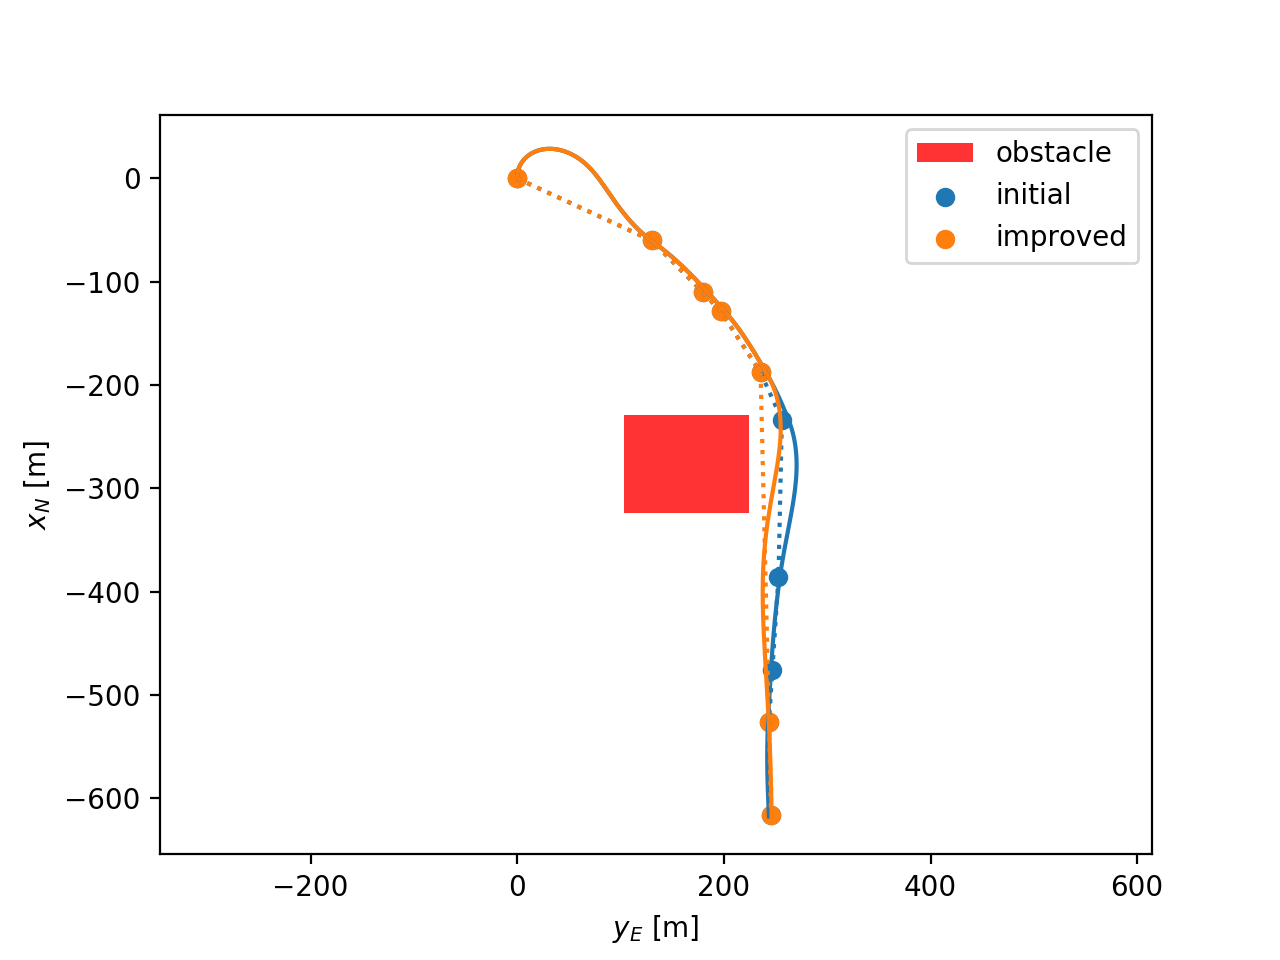
\includegraphics[width=\linewidth]{fig/sol_improved}
        \caption{Trajectory length reduction by eliminating waypoints. $x_0=(0,0,0\degree)$, $x_g=(-615, 245, 180\degree)$.}
        \label{fig:imp}
    \end{center}
\end{figure}

\section{Heuristic function}
As discussed in Section \ref{sec:a-star}, the choice of heuristic function is 
crucial in achieving good performance of the planner. The goal of the heuristic function is to estimate the 
length of the shortest air-relative path from an initial state $x_0$ to a final state $x_g$.

\subsection{Cost estimation for straight line-segments}\label{sec:straight_path_heuristic}
When following a straight line-segment in wind the distance travelled by the \ac{uav} relative to the air will be different from the distance relative to the ground. Assuming that the heading $\psi$ has converged to $\wca$, 
the speed of the \ac{uav} along the current reference line in the inertial frame is given by 
\begin{equation}
    V_{\parallel}=\cos\psi_s(\airspd\cos\wca+\windspd\cos\winddir) + \sin\psi_s(\airspd\sin\wca+\windspd\sin\winddir)
\end{equation}
This means that the time it takes for the \ac{uav} to travel along the line is equal to 
\begin{equation}
    t=\frac{\|\vec{p}_{i+1}-\vec{p}_i\|}{V_\parallel}
\end{equation}
where $\vec{p}_{i}$ and $\vec{p}_{i+1}$ are the start and end waypoints of the line. Thus, the distance 
travelled relative to the air is equal to 
\begin{equation}
    s_a=V_at=\frac{\airspd}{V_\parallel}\|\vec{p}_{i+1}-\vec{p}_{i}\|
\end{equation}
and $s_a$ provides a good heuristic estimate for traveling along a straight line-segment assuming that $\psi(x_0)=\psi(x_g)=\wca$.
This also implies that the Euclidean distance $\|\vec{p}_{i+1}-\vec{p}_{i}\|$ is not an admissible heuristic if 
$\airspd/V_\parallel<1$.

\subsection{Cost estimation for arbitrary initial and final heading}
Estimating the cost for traveling between states with arbitrary $\psi_0$ and $\psi_g$ is a more challenging problem than straight line-segments.
Methods to calculate such time-optimal paths in the presence of wind are given in both \cite{optimal_path_target} and \cite{optimal_path_trochoidal}, 
but since there is no analytical solution in all cases these methods rely on numerical root-finding techniques.
Computing these values every time an heuristic estimate is needed was deemed infeasible due to the high computational cost.

When the heuristic cannot be calculated in real-time, an option is to use a \ac{hlut} as discussed in Section \ref{sec:hlut}. By using the generated 
inputs $\inputs$ when calculating costs stored in the \ac{hlut}, these directly correspond to the true cost-to-go. However, a drawback of 
using a \ac{hlut} is that the wind speed $\windspd$ affects the cost, and thus different values of $\windspd$ require different \acp{hlut}. 

To estimate the cost of queries not stored in the \ac{hlut}, these queries can be projected as shown in Figure \ref{fig:hlut_proj}. The total heuristic value can then be estimated as 
\begin{equation}
    \tilde{h}(x, x_g) = h_{\ac{hlut}}(x, x_p) + h_s(x_p, x_g)
\end{equation}
where $h_s(x, \tilde{x})$ is the estimated cost for a straight line-segment.
\begin{figure}
    \begin{center}
        \begin{tikzpicture}
            \draw (-2, -2) rectangle (2, 2);

            \draw[my_v] (0,0) -- node[at end, below]{$y_E$} (1,0);
            \draw[my_v] (0,0) -- node[at end, left]{$x_N$} (0,1);

            \node[point] at (0,0){};
            \node[below] at (0,0){$x$};

            \node[point] at (2,1){};
            \node[above] at (2,1){$x_p$};
            \draw (0,0) -- node[midway, below, anchor=north west]{$h_{\ac{hlut}}(x, x_p)$} (2,1);

            \node[point] at (4,2){};
            \node[above] at (4,2){$x_g$};
            \draw[dashed] (2,1) -- node[midway,below, anchor=north west]{$h_s(x_p,x_g)$} (4,2);

            \node[anchor=west] at (-1.8,-1.75){\ac{hlut} available};
        \end{tikzpicture}
    \end{center}
    \caption{Projection of queries on \ac{hlut}}
    \label{fig:hlut_proj}
\end{figure}

\subsubsection{Wind variation effects on the heuristic}
If the actual wind speed $\tilde{\windspd}$ is different from the wind speed $\windspd$ used during planning, this 
might affect the admissibility of the heuristic. 
To study this effect, consider traveling along a straight path segment of length $\Delta s=\|x-\tilde{x}\|$ under the assumptions in Section \ref{sec:straight_path_heuristic}. 
An admissible heuristic is then 
\begin{equation}
    \tilde{h}(x, \tilde{x})=\frac{\airspd}{V}\Delta s
\end{equation}
where $V$ is the velocity in the inertial frame. Wind has the largest effect on $V$ when traveling in direct tailwind or headwind, and in those cases $V=\airspd\pm \tilde{\windspd}$. The 
heuristic function $h(x, \tilde{x})$ used during planning is the same but with $V=\airspd\pm \windspd$. The ratio between the admissible and actual heuristics becomes
\begin{equation}\label{eq:wind_heuristic_eps}
    \epsilon = \frac{h}{\tilde{h}} = \frac{\airspd \pm \tilde{\windspd}}{\airspd \pm \windspd}
\end{equation}
where the signs in the numerator and denominator must be equal. From Section \ref{sec:sub_optimal} we know that the heuristic is not admissible if 
$\epsilon>1$ which is the case if $\tilde{\windspd}>\windspd$ when traveling in tailwind, or $\tilde{\windspd}<\windspd$ when traveling in headwind.
In these cases, using this heuristic estimate is analouge to using an inflated heuristic with inflation factor $\epsilon$. Moreover, the effects of using an incorrect wind estimate will be more significant if the 
magnitude of $\tilde{\windspd}$ is close to that of $\airspd$.